Load-balancing problems can be formulated in many ways. This is
especially true for the case addressed in this paper where the
load-balancer should distribute the load to adaptive entities, that
play a role by themselves in adjusting to the current situation. This
section discusses the characteristics of the considered infrastructure
and clearly formulate the problem under analysis.

\begin{figure}[t]
  \centering 
  \usetikzlibrary{arrows}
\usetikzlibrary{automata}
\usetikzlibrary{positioning}
\usetikzlibrary{backgrounds}
\usetikzlibrary{fit}

\tikzset{
    state/.style={
           rectangle,
           rounded corners,
           draw=black, very thick,
           minimum height=0.6cm,
           minimum width=1.3cm,
           inner sep=3pt,
           text centered,
           node distance=1.8cm,
           },
    process/.style={
           rectangle,
           rounded corners,
           draw=black, very thick,
           minimum height=0.6cm,
           minimum width=1.3cm,
           inner sep=3pt,
           text centered,
           %node distance=1cm,
           },
    newprocess/.style={
           rectangle,
           rounded corners,
           draw=black, very thick,
           fill=lightgray,
           minimum height=0.6cm,
           minimum width=1.3cm,
           inner sep=3pt,
           text centered,
           %node distance=1cm,
           },
    processplaceholder/.style={
           minimum height=0.6cm,
           minimum width=1.3cm,
           %inner sep=3pt,
           text centered,
           %node distance=1cm,
           },
    closerstate/.style={
           rectangle,
           rounded corners,
           draw=black, very thick,
           minimum height=0.5cm,
           minimum width=5.35cm,
           inner sep=3pt,
           text centered,
           node distance=1.1cm,
           },
    abovish/.style={
           rectangle,
           rounded corners,
           draw=none,
           minimum width=1.3cm,
           text centered,
           node distance=1.3cm,
           },
    supercloserstate/.style={
           rectangle,
           draw=none,
           minimum height=0.2cm,
           minimum width=6.9cm,
           node distance=1cm,
           },
}

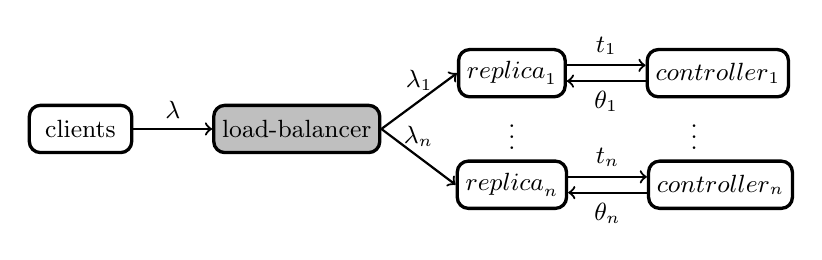
\begin{tikzpicture}[font=\small]
\tikzstyle{surround} = [fill=black!20,very thick,draw=black,rounded corners, inner sep=5pt,]
\tikzstyle{surroundblue} = [fill=blue!20,very thick,draw=black,rounded corners, inner sep=5pt,]
\tikzstyle{surroundyellow} = [fill=yellow!20,very thick,draw=black,rounded corners, inner sep=5pt,]
\tikzstyle{external} = [fill=none,very thick,draw=black,rounded corners, inner sep=15pt,]

% clients
\node[process] (clients){clients};

% load-balancer
\node[newprocess, right=1cm of clients] (lb){load-balancer};

% servers
\node[processplaceholder, right=1cm of lb] (replicaI) {$\vdots$};
\node[process, above=0cm of replicaI] (replica1) {$\text{replica}_1$};
\node[process, below=0cm of replicaI] (replicaN) {$\text{replica}_n$};

% controllers
\node[processplaceholder, right=1cm of replicaI] (controllerI) {$\vdots$};
\node[process, right=1cm of replica1] (controller1) {$\text{controller}_1$};
\node[process, right=1cm of replicaN] (controllerN) {$\text{controller}_n$};

% clients to lb
\draw[thick,->] (clients.east) -- (lb.west) node[midway, above] {$\lambda$};

% lb to replicas
\draw[thick,->] (lb.east) -- (replica1.west) node[midway, above] {$\lambda_1$};
\draw[thick,->] (lb.east) -- (replicaN.west) node[midway, above] {$\lambda_n$};

% replica to controllers
\draw[thick,->] ([yshift=+1mm]replica1.east) -- ([yshift=+1mm]controller1.west) node[midway, above] {$t_1$};
\draw[thick,<-] ([yshift=-1mm]replica1.east) -- ([yshift=-1mm]controller1.west) node[midway, below] {$\theta_1$};
\draw[thick,->] ([yshift=+1mm]replicaN.east) -- ([yshift=+1mm]controllerN.west) node[midway, above] {$t_n$};
\draw[thick,<-] ([yshift=-1mm]replicaN.east) -- ([yshift=-1mm]controllerN.west) node[midway, below] {$\theta_n$};

\end{tikzpicture}
 
  \caption{Architecture of a brownout-compliant cloud application
    featuring multiple replicas.}
    \vspace{-6mm}
  \label{fig:architecture}
\end{figure}

Figure~\ref{fig:architecture} illustrates the software architecture
that is deployed to execute a brownout-compliant application composed
of multiple replicas. Despite the modifications needed to make it
brownout-compliant, the architecture is widely accepted as the
reference one for cloud applications~\citep{Barroso09}.

In a generic load-balancing infrastructure, clients generate traffic
to the cloud application at an unknown but measurable rate
$\lambda$. The traffic is directed to a load-balancer that demultiplexes it,
sending requests to the $n$ different replicas. Each client request
directed to the application is received by the load-balancer, that
sends it to a replica. The replica produces the response and send it
back to the load-balancer, which forwards it to the original
client. We measure the \textbf{response time} of the request as the
time spent within the replica, assuming negligible time is taken for
the load-balancer execution and for the routing itself. Also, since
the responses are routed back to the load-balancer, it is possible to
piggy-back information that can guide load-balancing decisions.

Each replica $i$ receives a fraction $\lambda_i$ of the incoming
traffic and implements the application logic. More specifically, each
replica receives requests at a rate $\lambda_i = w_i \cdot \lambda$,
such that $\sum_{i} w_i = 1$. In this case, the load balancer simply
computes the \textbf{replica weights} $w_i$ according to its
load-balancing policy.

Special to our case is the presence of a controller within each
replica~\cite{cloudish-tr}. This controller takes care of adjusting
the percentage of requests served with the optional components enabled
based on the measured response time of the requests served by the
replica. The controller for replica $i$ receives a statistic on the
replica response times. The average, $95$-th percentile or maximum value can be used, 
depending the requirements of the application.
Here we use the $95$-th percentile of
response times. Based on that, the controller computes the percentage 
$\theta_i$ of requests that should be served with optional components 
during the next control interval.

As given by the brownout paradigm, a replica $i$ responds to requests either partially, where
only mandatory content is included in the reply, or fully, where both
mandatory and optional content is included. This decision is taken independently for
each request, based on a Bernoulli trial, with probability $\theta_i$ for success.
The service rate for a
partial response is $\mu_i$ while a full response is generated with a
rate $M_i$. Obviously, partial replies are faster to compute than full
ones, since the optional content does not need to be prepared, hence,
$\mu_i > M_i$. Assuming the replica is not saturated, it serves
requests fully at a rate $\lambda_i \cdot \theta_i$ and partially at a
rate $\lambda_i \cdot (1-\theta_i)$.

Many alternatives can be envisioned on how to extend existing load
balancers to deal with brownout-compliant applications. As a first architecture,
the load-balancer does not know anything about the current state
of the system but can inspect the requests and the responses, and
receives information about how many of them have been executed with
the optional components turned on. This would give it an estimation of
the probability of executing optional code $\theta_i$ per replica but
not the certainty of its current value, due to the probabilistic
setup.

As a second architecture, the load-balancer does not know anything about the
state of the system and cannot inspect the requests because this would
load the architecture unacceptably, therefore it can try to estimate
the probability of executing optional code based on the time needed to
compute the response --- clearly, a request with optional code enabled
would take longer than one without it. The estimate of $\theta_i$ in
this case would be less accurate than in the previous architecture.

In the third architecture, the load-balancer receives information about
$\theta_i$ from the replicas. This solution results in less
computationally intensive load-balancers but requires additional
communication. The overhead, however, is very limited, since only one
value would be reported per replica. For the purpose of this paper, we
assume that to aid load-balancing decisions, each replica piggy-backs
the current value of $\theta_i$ through the reply, so that this value
can be observed by the load-balancer, limiting the overhead. The
load-balancer does not have any knowledge on \emph{how} each replica
controller adjusts the percentage $\theta_i$, it only knows the
reported value.

\str{Comment on ``separation'' and ``fast/slow dynamics''. 0.2 seconds
  is the period of the replica controller while 1 second is the
  load-balancer one.}

Given this last architecture, we want to solve the problem of designing a
{\bf load-balancer policy}. Knowing the values of $\theta_i$ for each
replica $i \in [1, n]$ and the current (assumed constant) arrival rate
$\lambda$, a load-balancer should compute the values of the weights
$w_i$ such that
\begin{equation}
\sum_{i} \lambda w_i \theta_i = \lambda \sum_i w_i \theta_i
\label{eq:objective}
\end{equation}
is maximized. In other words, the load-balancer should maximize the
amount of requests served with the optional part enabled. In practice,
this would also maximize the application owner's
revenue~\cite{cloudish-tr}.
